\subsection{Jetson Orin Nano Integration}

This section is from the spring 2023 semester. During the integration of the Jetson Orin Nano and the drone system, we encountered unexpected issues and device malfunctions, which prevented us from incorporating the YOLOv5 detection model and MiDaS depth estimation model into the system. Instead, we utilized the OpenCV library and developed a QR code tracking script that enables the drone to detect QR codes and rotate to track them. 

\begin{figure}[H]
    \centerline{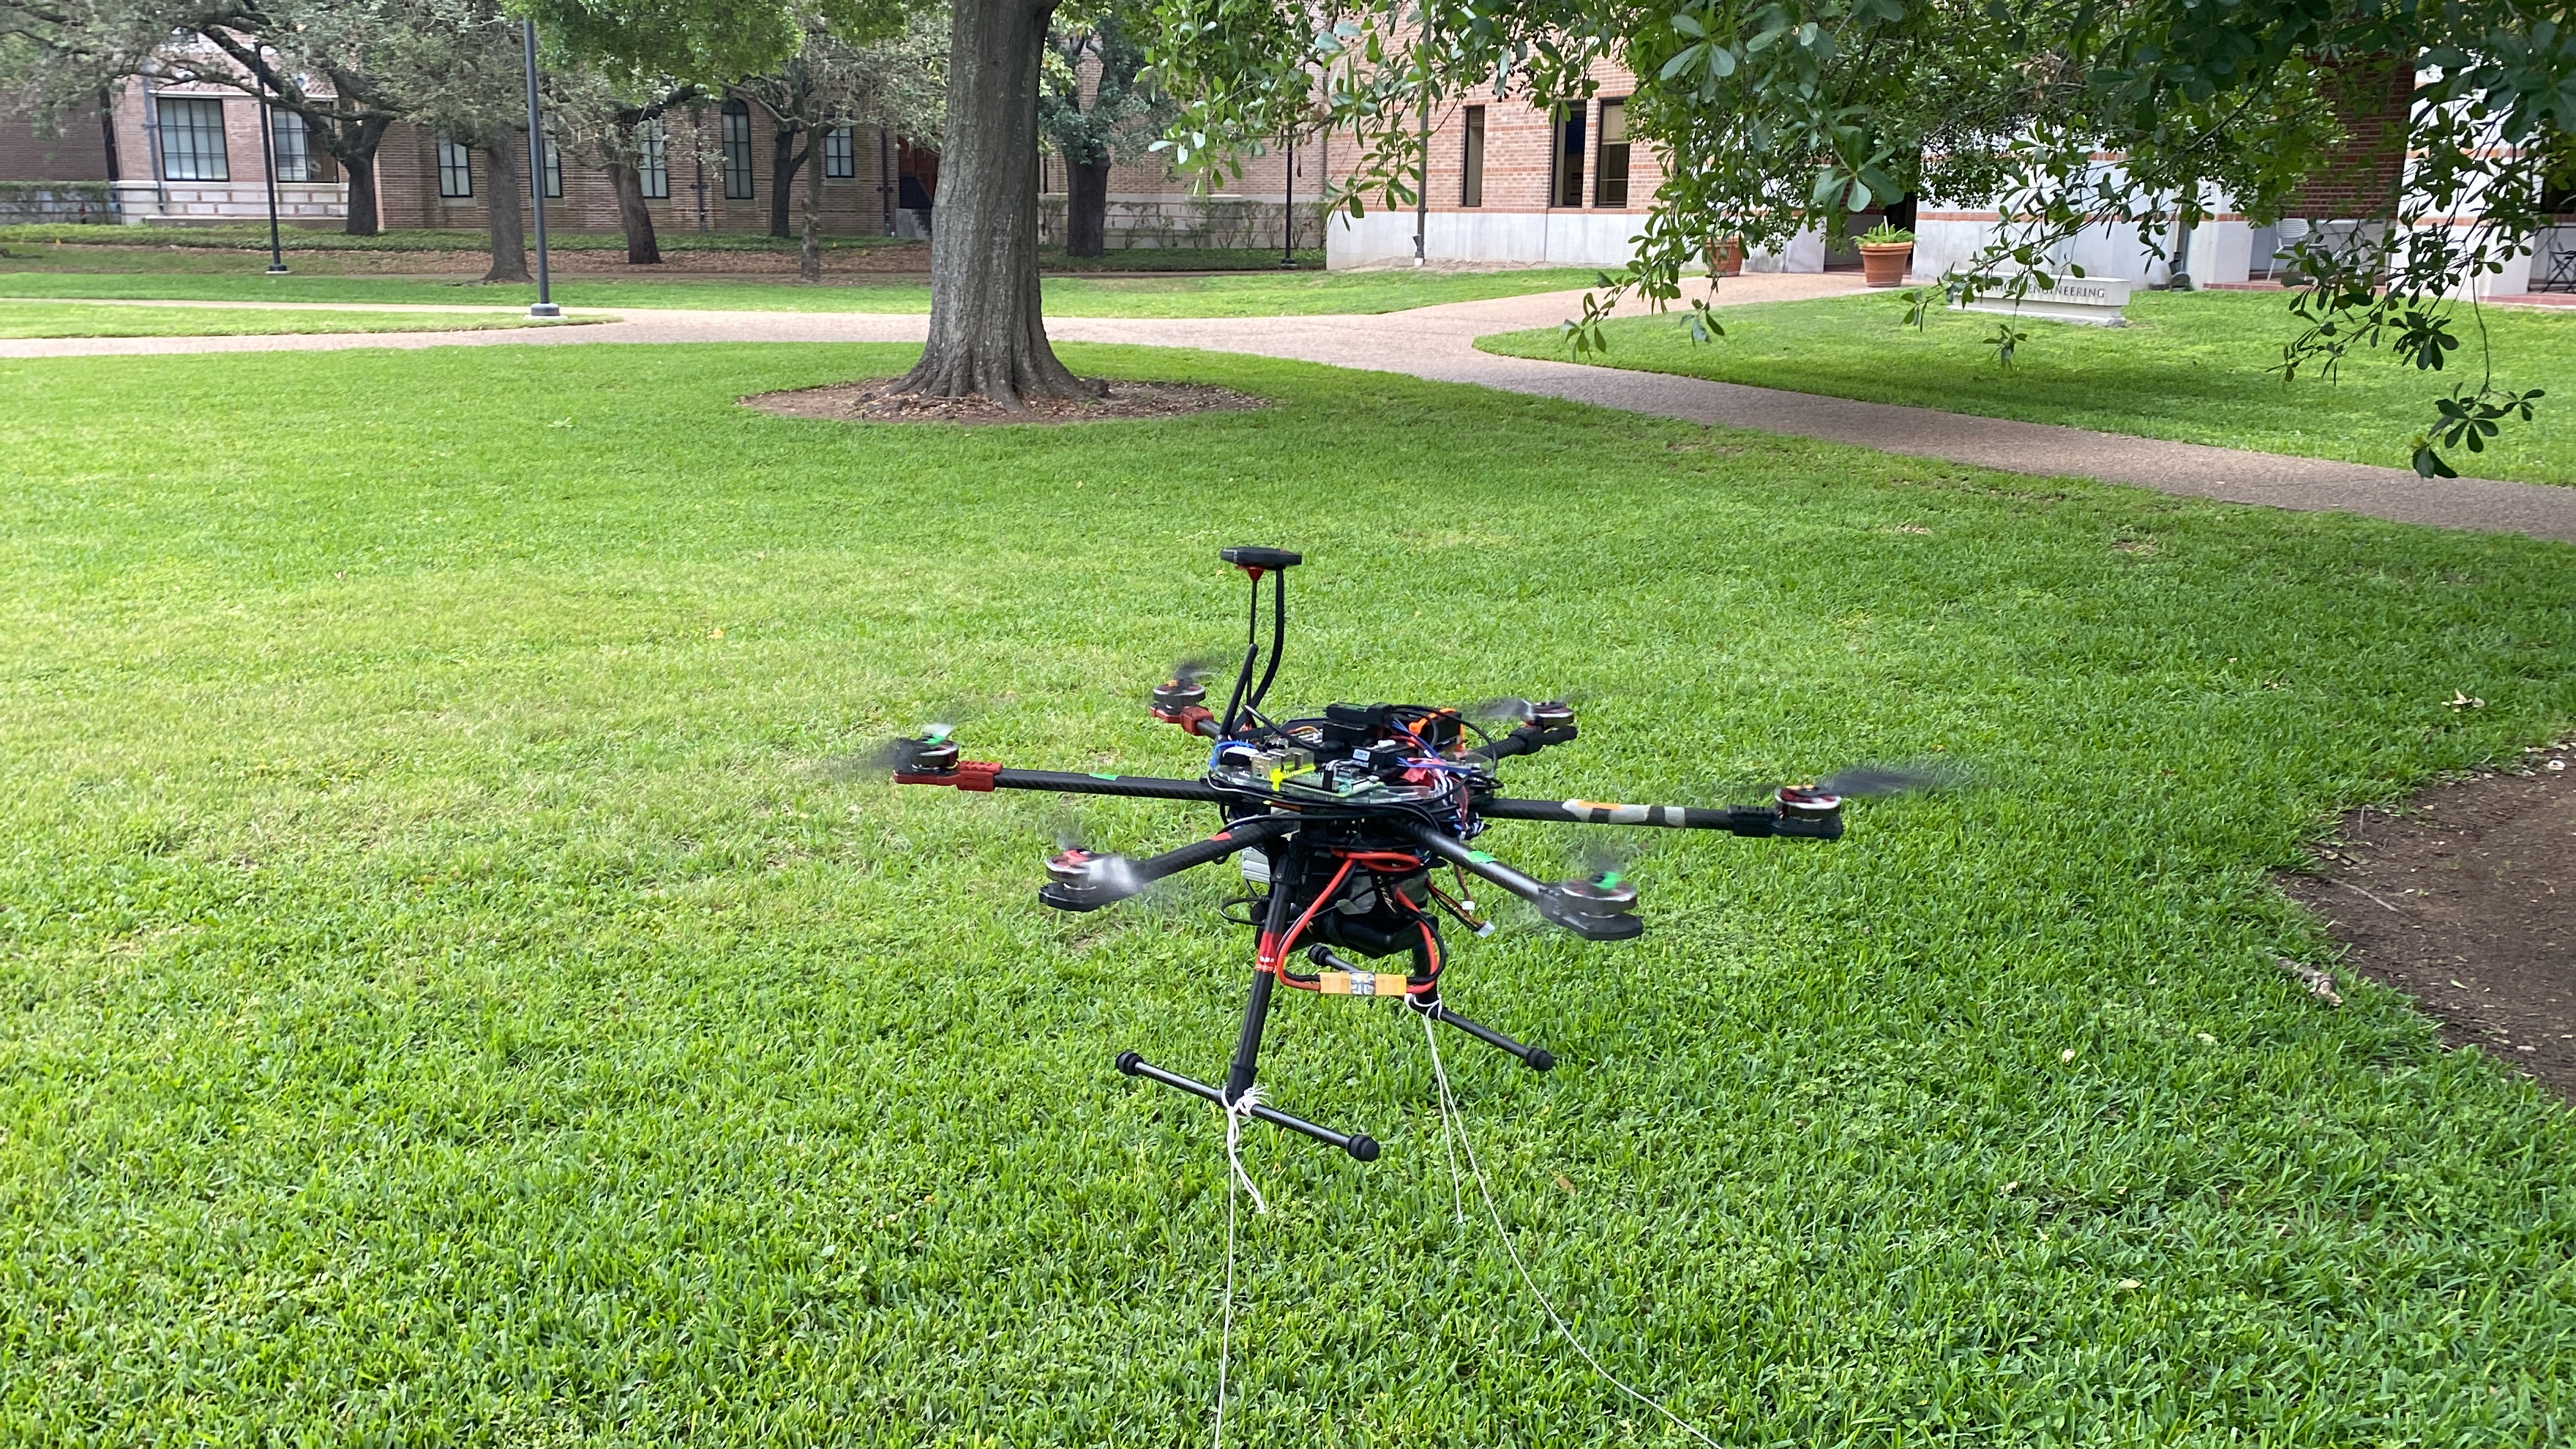
\includegraphics[width=0.5\textwidth]{Figures/Results/Drone_Hover.JPG}}
    \caption{Hover drone in the air operated by Jetson Orin Nano.}
    \label{fig3b1}
\end{figure}

Before implementing this experiment, we tested several other simple movement scripts. Fig. ~\ref{fig3b1} shows the drone hovering successfully in the air for the first time, while Fig. ~\ref{fig3b2} shows the final experiment in which the drone hovers in the air and tracks the QR code. This experiment was conducted in a real-world environment.

\begin{figure}[H]
    \centerline{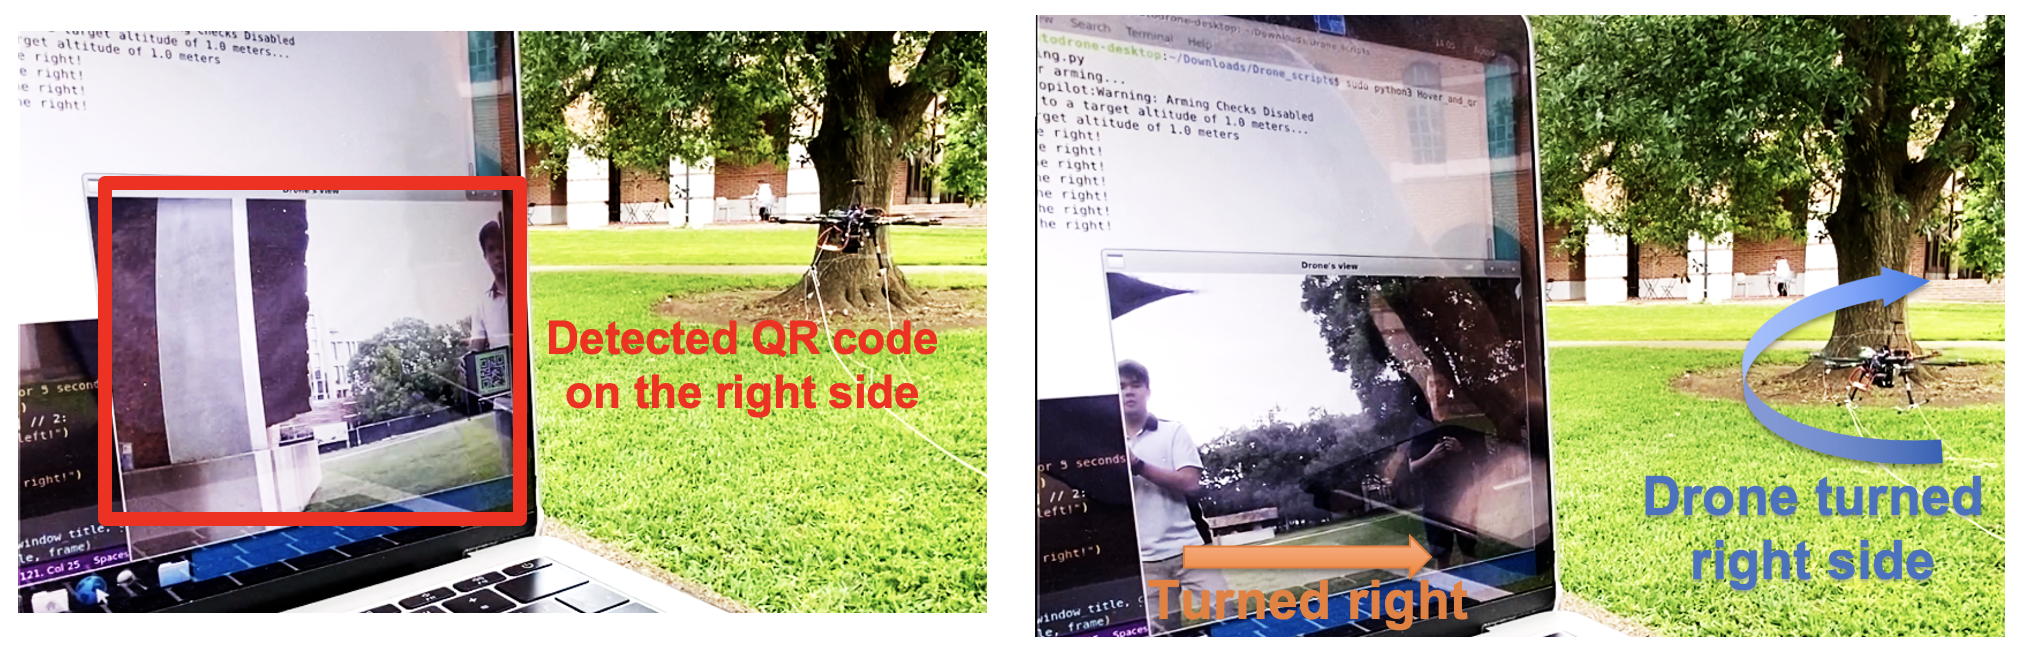
\includegraphics[width=0.5\textwidth]{Figures/Results/QR_code_Tracking_Successfully.png}}
    \caption{QR code tracking results on Jetson Orin Nano.}
    \label{fig3b2}
\end{figure}

This section below is from the fall 2023 semester.
% TODO: Add Stuff

For this semester, the Robot Operating System (ROS)  was successfully integrated in the Jetson Orin Nano, establishing a robust connection with the Ardupilot Flight Control. This integration enabled the comprehensive control and monitoring of the drone system, laying a foundational framework for advanced drone operations. This integration enabled the accessibility and functionality of both external (camera, LiDAR) and internal (GPS, IMU, barometer) sensors within the flight control unit. These sensors now effectively contribute fundamental flight and awareness data to the system. Additionally, the project made strides in enabling motion control of the drone through ROS nodes, facilitated by the effective communication between the Jetson Orin Nano and the flight control unit via MAVROS/MAVPROXY. However, the current motion control system is somewhat limited by the constraints of existing wrapped functions, highlighting an area for future improvement. The project team anticipates enhancing this aspect by developing custom functions using underlying FCU code for more direct interaction with the flight control system.

The project also achieved considerable success in the area of multiple sensor fusion. The integration of camera and lidar sensors was not only successfully accomplished but also optimized to ensure efficient data streaming to ROS topics. This development provided the drone with basic yet powerful perception capabilities. This fusion effectively combined environmental imaging with depth estimation, offering a more comprehensive understanding of the drone's surroundings, as shown in Fig. ~\ref{fig3b3} and  
Fig. ~\ref{fig3b4}. Additionally, the team managed to establish and visualize the spatial orientation of the sensors relative to the drone body using RVIZ, thereby enhancing the drone's spatial awareness by rearranging the transformation between the frames. A significant reduction in the latency of data capture was achieved by transitioning to more efficient capture packages. The project aims to further refine the range and angle mapping between the camera and lidar sensors and develop additional applications to enhance the drone's perception capabilities.

\begin{figure}[H]
    \centerline{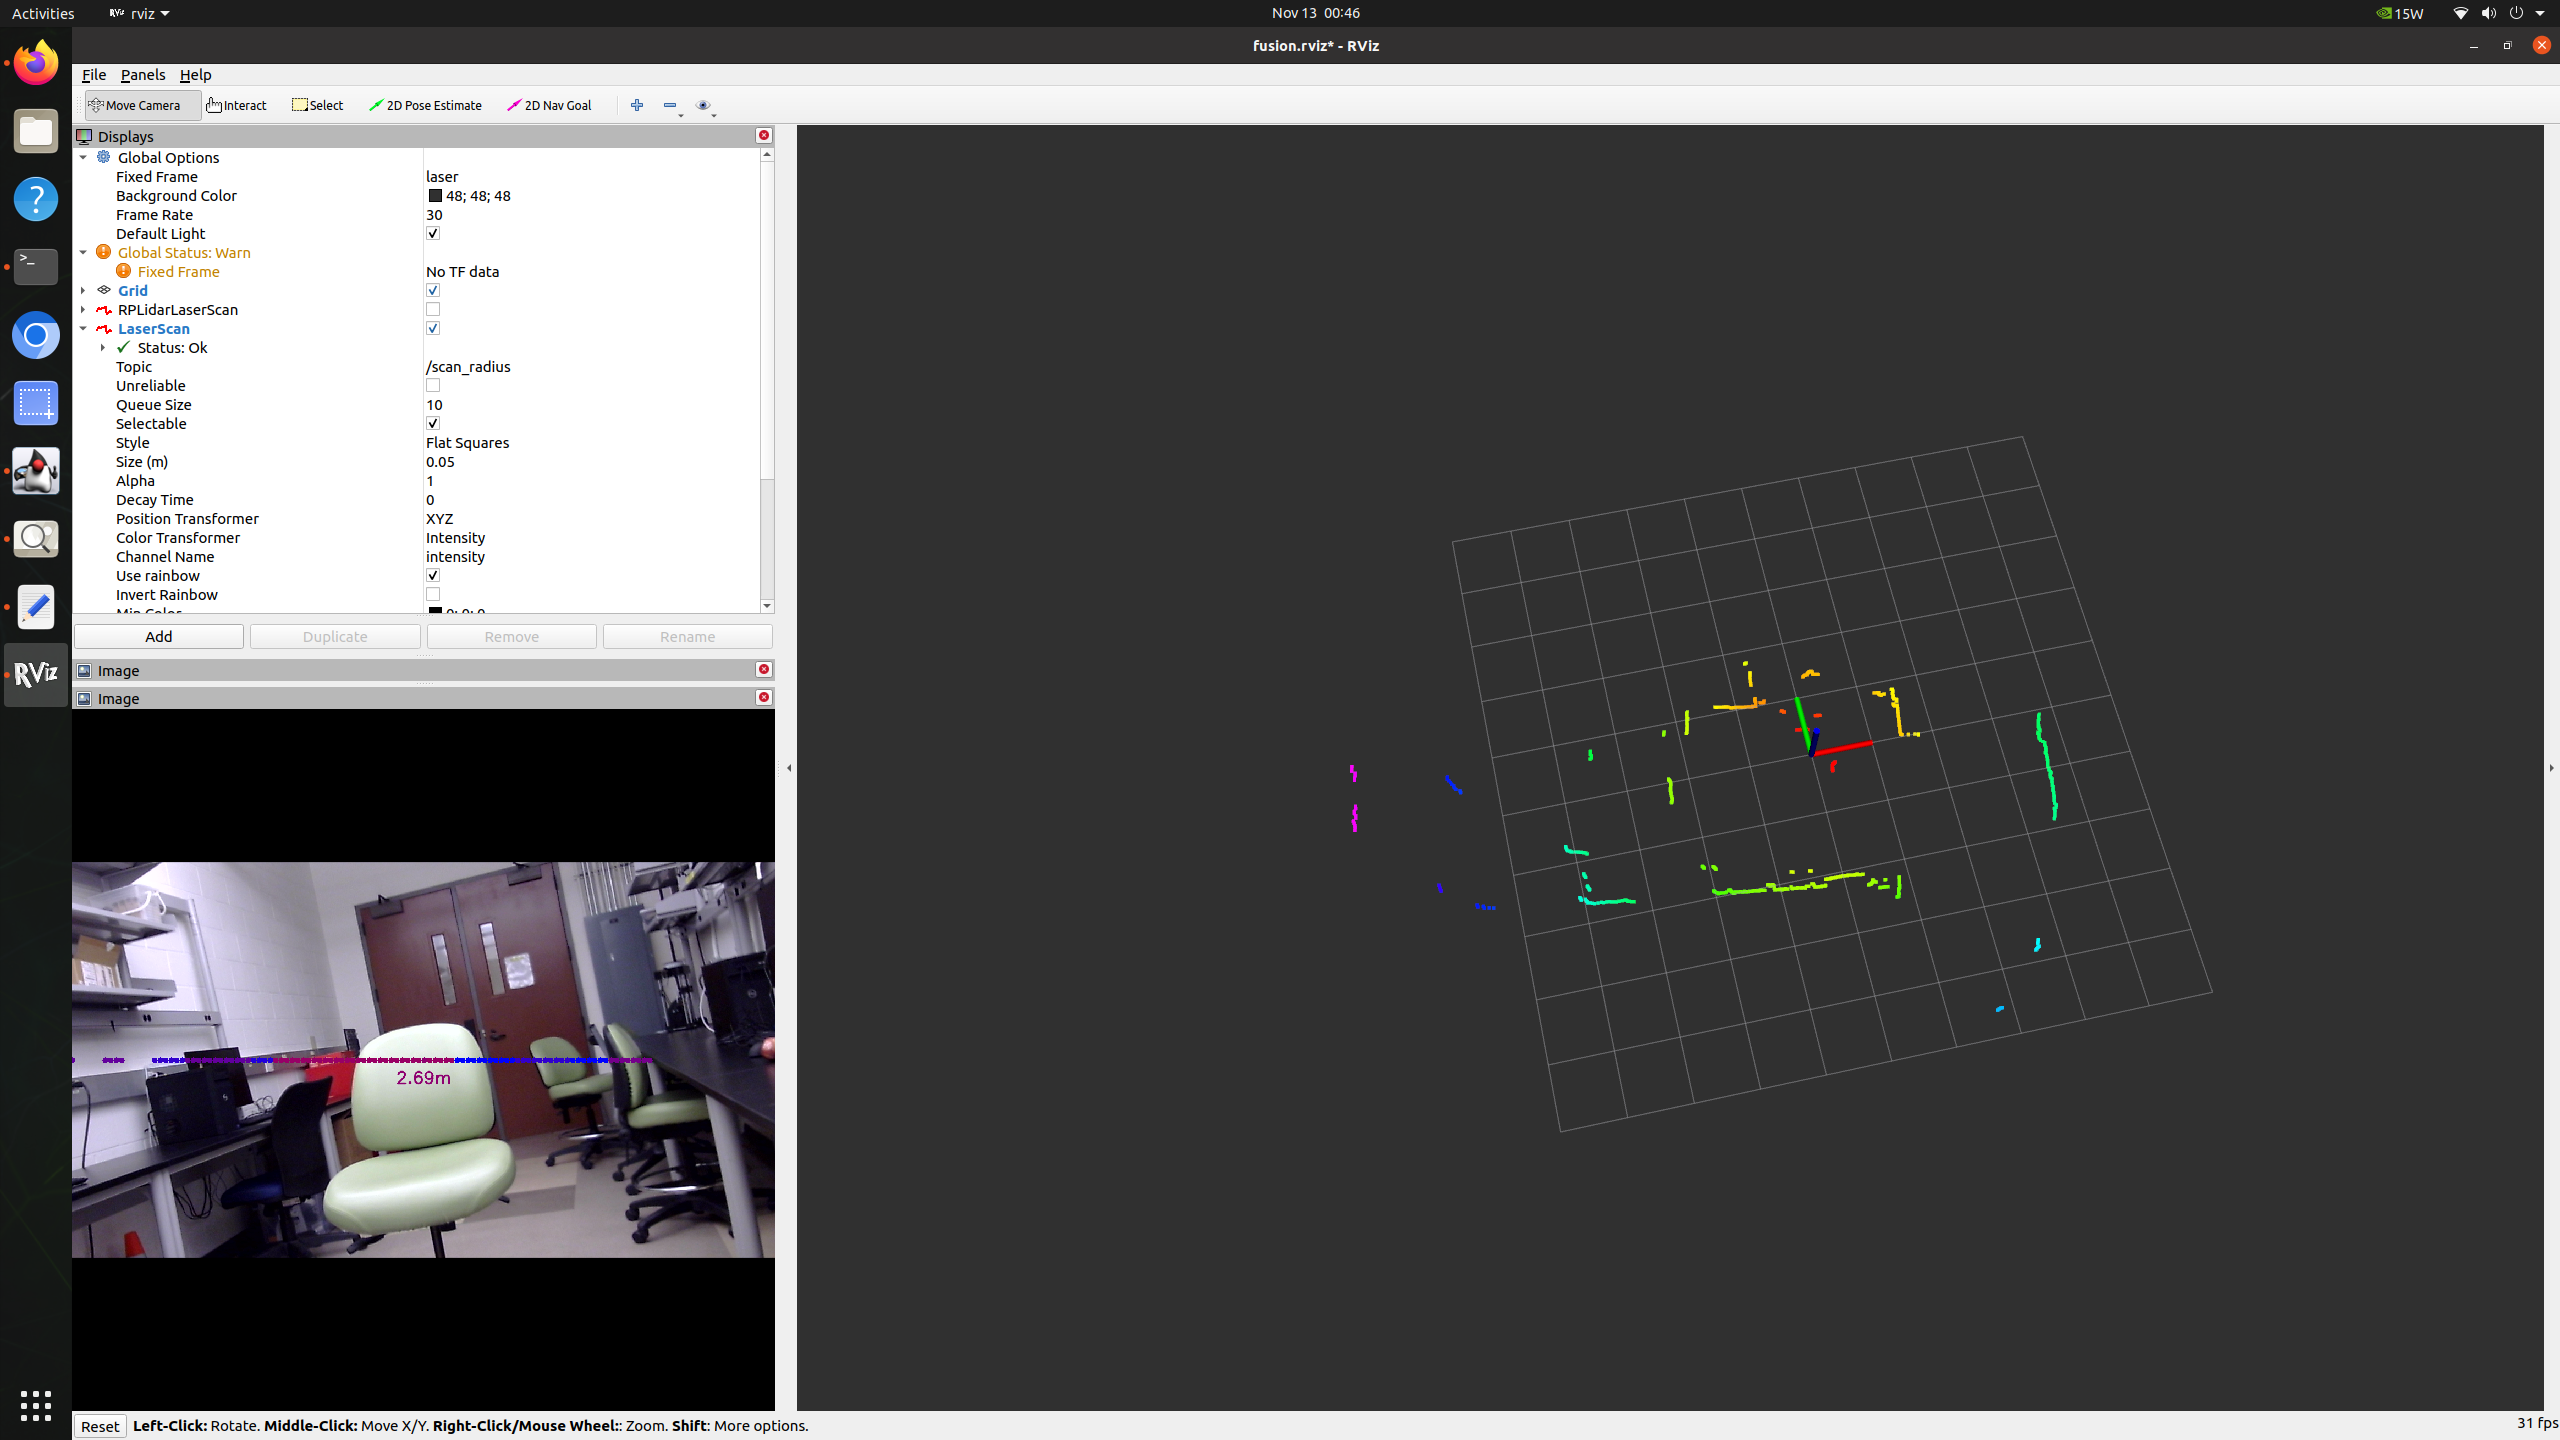
\includegraphics[width=0.5\textwidth]{Figures/Results/fusion5_with_distance.png}}
    \caption{Camera-LiDAR Fusion with Distance Estimation(Close).}
    \label{fig3b3}
\end{figure}


\begin{figure}[H]
    \centerline{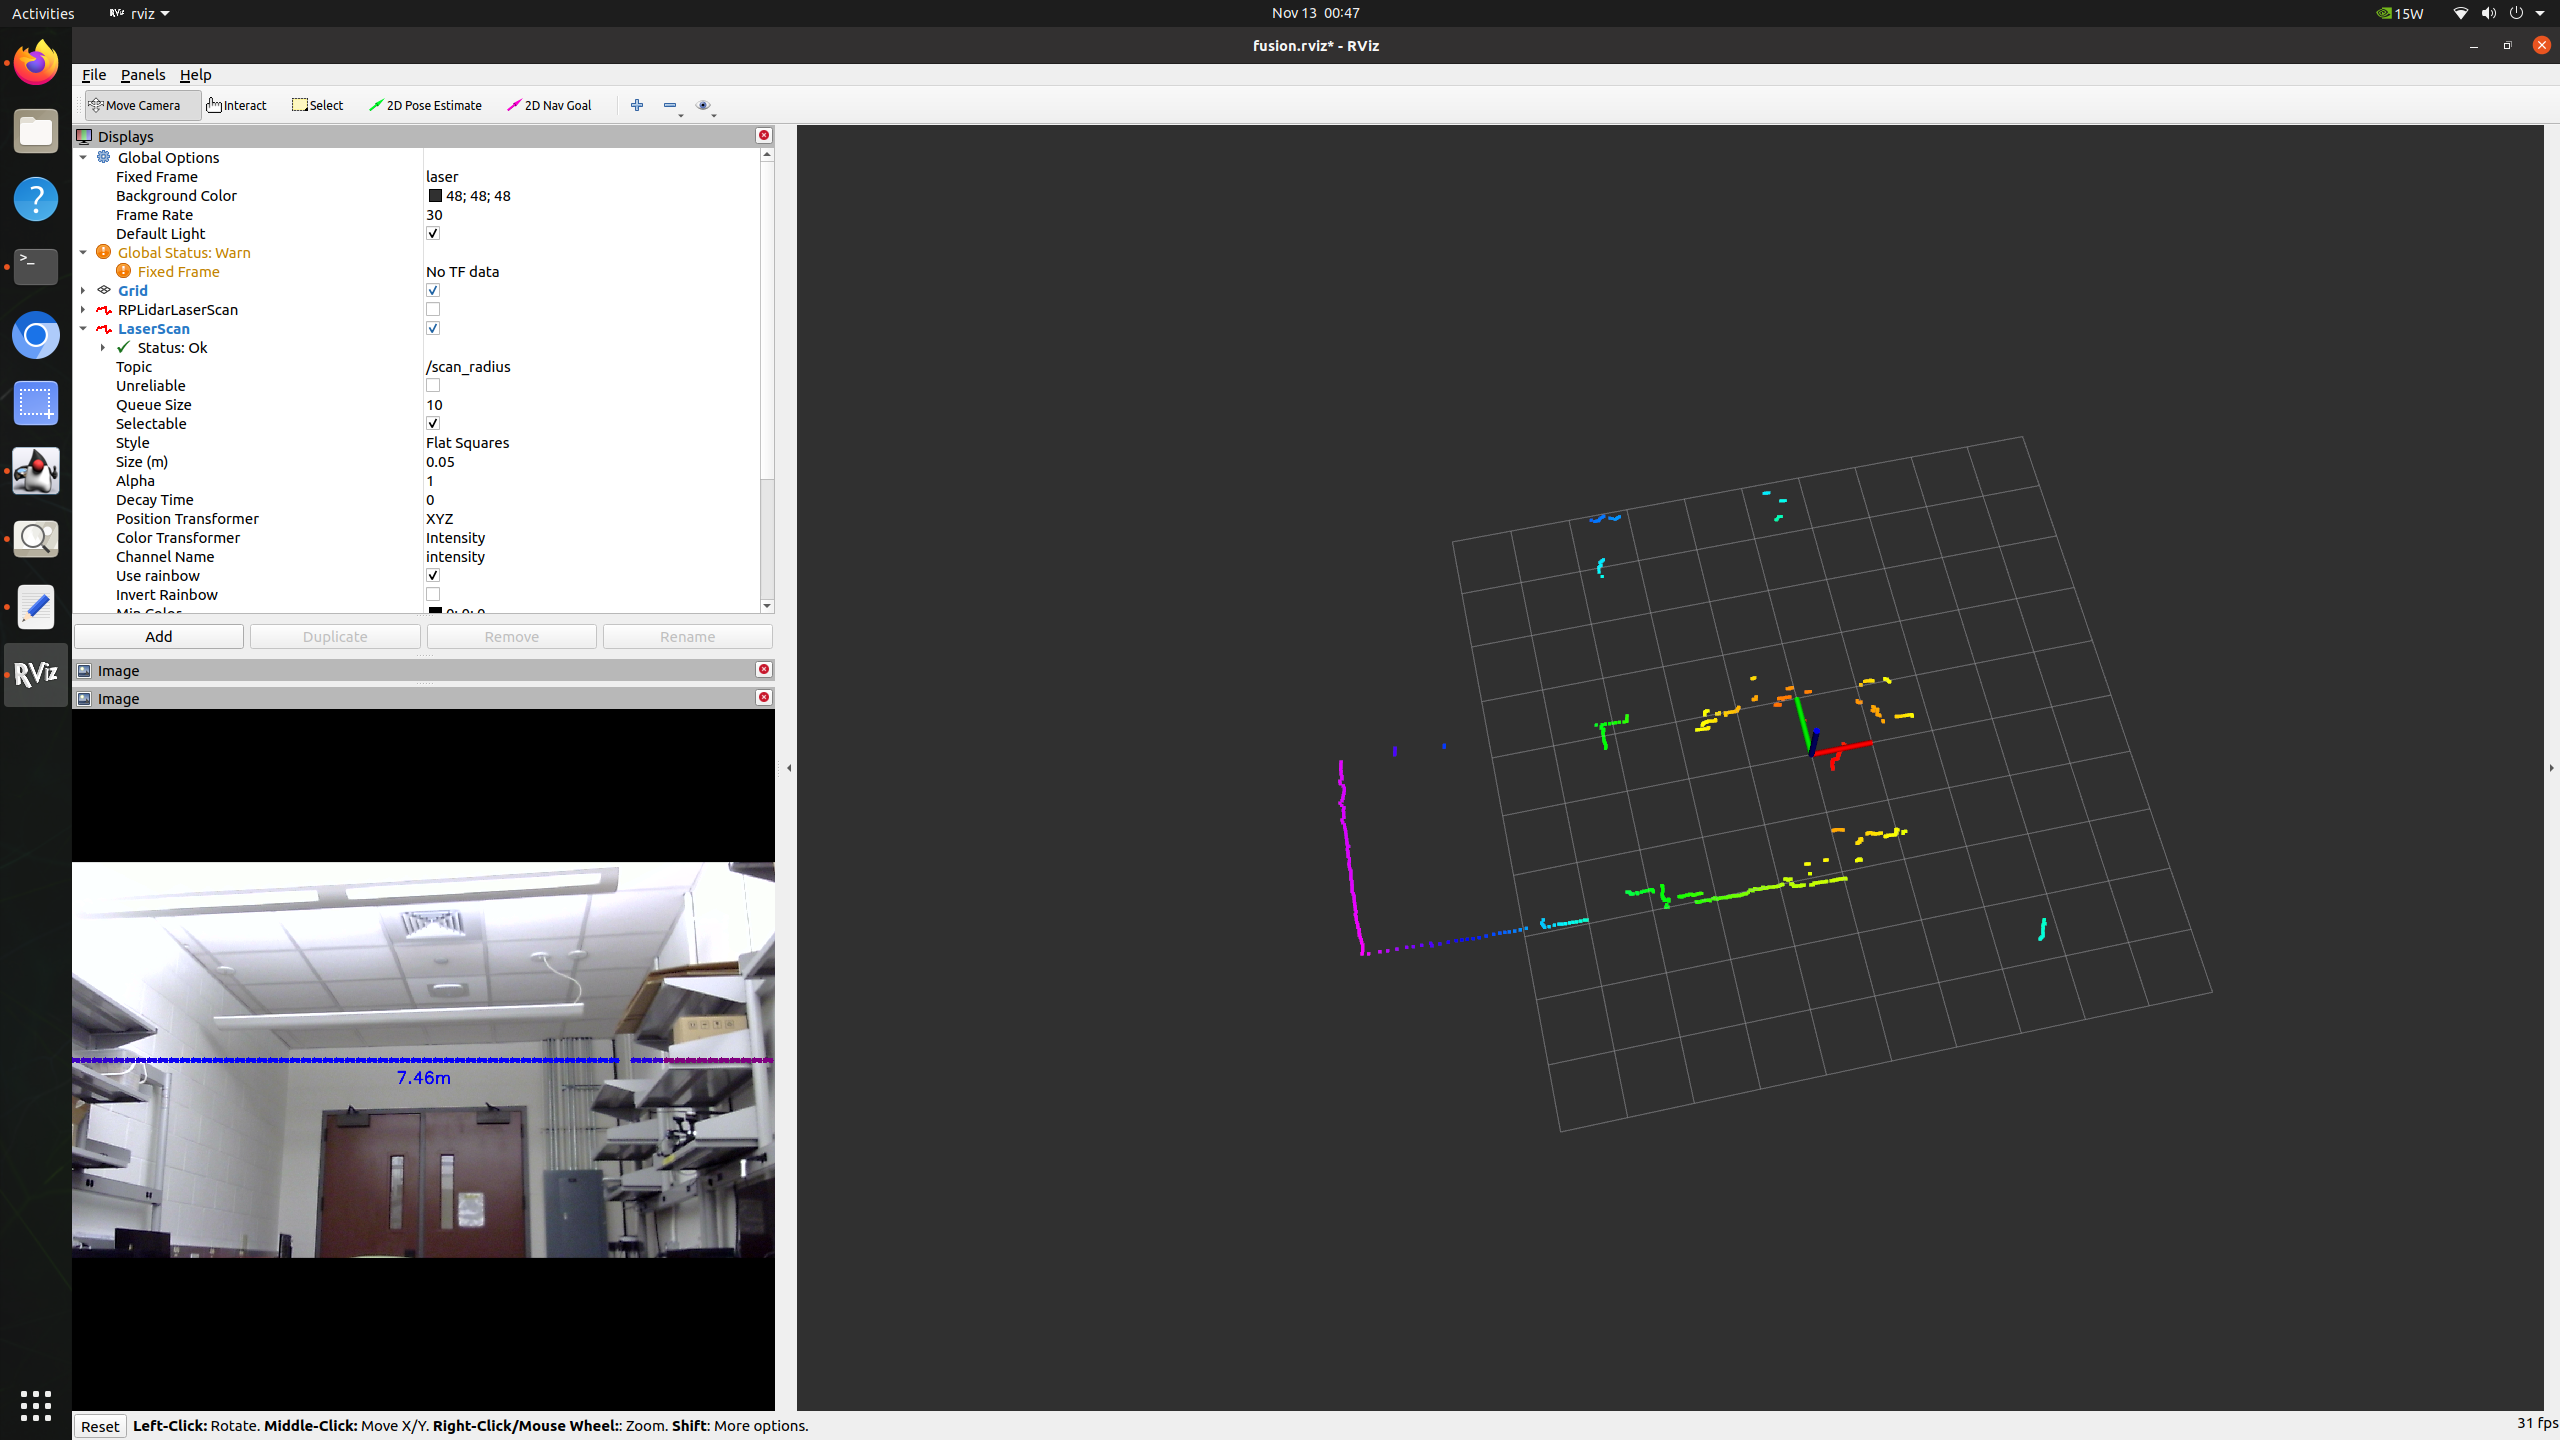
\includegraphics[width=0.5\textwidth]{Figures/Results/fusion6_with_distance.png}}
    \caption{Camera-LiDAR Fusion with Distance Estimation(Far).}
    \label{fig3b4}
\end{figure}

In the realm of on-board algorithm development, the project made substantial progress, aligning closely with initial objectives, although some areas still under development. The obstacle avoidance and tracking algorithms, critical for the drone's navigation and environmental interaction, were developed and tested in a simulator. These preliminary versions demonstrated basic environmental awareness, but full functionality is pending due to a limited understanding of the internal workings of the Flight Control Unit (FCU). However, the mission planning algorithm, a vital component for autonomous drone operations, is still in the development phase. The team's focus is currently on enabling the drone's autonomous sensing and movement in controlled scenarios, which is expected to significantly advance the drone’s operational capabilities.


